\documentclass[11pt]{article}
\usepackage[paperwidth=8.5in, paperheight=11in]{geometry}
\usepackage{algorithm}
\usepackage{algorithmicx}
\usepackage[noend]{algpseudocode}

\usepackage{../tjimo}

\newcommand{\sevenpoints}{Time limit: 45 minutes.}
\newcommand{\righthead}{\fdbox{Round}{Power}}

\begin{document}

\section{What is a Graph?}

You might have heard of a graph in your math class as a plot with an $x$ and $y$ axis. Or maybe in science you looked at
bar graphs and pie graphs. Maybe in history you took a look at line graphs. But the graphs we are going to talk about today
are none of the above.

\subsection{Some Introduction}

At its core, a \textit{graph} consists of two sets: a group of objects, and a group of connectors that each join two objects.

To gain insight into what a graph is, let's first consider flights that connect airports around the world.
We depend on airplanes to travel quickly and efficiently. When we want to travel between major cities,
like between D.C. and Boston, we can often take a single flight to make the trip. Enough people want to travel between
these two cities for it to be economical to offer a single flight between them.

However, it is not always the case that single-flight trips are economically feasible, either due to lack of demand
or due to needing to refuel. To travel from London to Yellowstone, for example, one must first stop in Atlanta, hop
on a connecting flight to Denver, and then finally travel to Yellowstone. Denver and Atlanta are what we call
hubs, since they are very large airports that accomodate heavy travel loads. To travel between smaller airports, we often
need to stop at one of these larger hubs.

\begin{center}
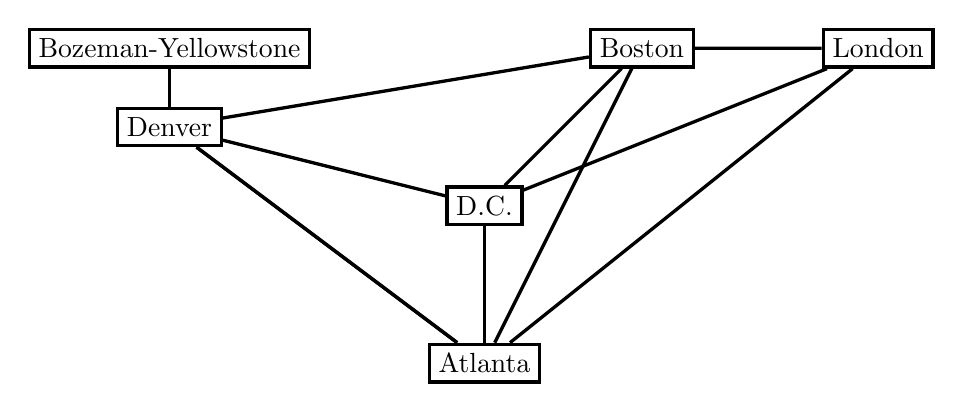
\begin{tikzpicture}[very thick,level/.style={sibling distance=70mm/#1}]
\draw (0, 0) node[draw, shape=rectangle] (a) {D.C.};
\draw (-4, 1) node[draw, shape=rectangle] (b) {Denver};
\draw (0, -2) node[draw, shape=rectangle] (c) {Atlanta};
\draw (2, 2) node[draw, shape=rectangle] (d) {Boston};
\draw (5, 2) node[draw, shape=rectangle] (e) {London};
\draw (-4, 2) node[draw, shape=rectangle] (f) {Bozeman-Yellowstone};
\draw (a) -- (b) -- (c) -- (d) -- (e);
\draw (b) -- (f);
\draw (c) -- (b);
\draw (a) -- (d);
\draw (b) -- (d);
\draw (a) -- (c);
\draw (c) -- (e);
\draw (a) -- (e);
\end{tikzpicture}
\end{center}

Our connections between our cities in the graph represent only direct connections between
cities, but from our diagram, we can still see it is possible to travel between any two
cities in our graph.

Neither the exact position of each city nor how connections might intersect 
matters. In other words, the way we draw a graph on paper does not change its properties, and for the most part
are not useful to us. The following is an equivalent graph:

\begin{center}
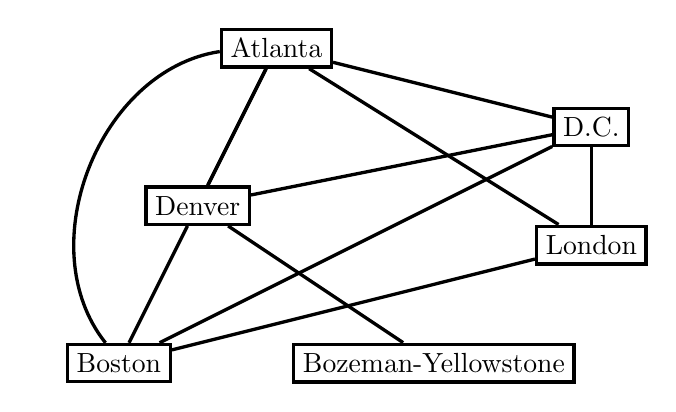
\begin{tikzpicture}[very thick,level/.style={sibling distance=70mm/#1}]
\draw (5, 3) node[draw, shape=rectangle] (a) {D.C.};
\draw (0, 2) node[draw, shape=rectangle] (b) {Denver};
\draw (1, 4) node[draw, shape=rectangle] (c) {Atlanta};
\draw (-1, 0) node[draw, shape=rectangle] (d) {Boston};
\draw (5, 1.5) node[draw, shape=rectangle] (e) {London};
\draw (3, 0) node[draw, shape=rectangle] (f) {Bozeman-Yellowstone};
\draw (a) -- (b) -- (c);
\path (c) edge [bend right=60] (d);
\draw (d) -- (e);
\draw (b) -- (f);
\draw (c) -- (b);
\draw (a) -- (d);
\draw (b) -- (d);
\draw (a) -- (c);
\draw (c) -- (e);
\draw (a) -- (e);
\end{tikzpicture}
\end{center}

The only characteristics of a graph we care about are the objects (in this case, cities) themselves, which we'll call \textit{vertices},
and the connections joining the objects, which we'll call \textit{edges}.

\subsection{Definition of a Graph}

We now have the background necessary to present the mathematical definition of a graph:

\begin{definition}
\label{def:graph}
A \textit{graph} $G(V,E)$ consists of a set of vertices $V$ and a set of edges $E$. 

\begin{center}
\begin{tikzpicture}[very thick,level/.style={sibling distance=70mm/#1}]
\draw (0, 0) node [vertex] (A) {$A$};
\draw (2, 1) node [vertex] (B) {$B$};
\draw (2, -1) node  [vertex] (C) {$C$};
\draw (4, 0) node [vertex] (D) {$D$};
\draw (A) -- (B);
\draw (B) -- (C);
\draw (C) -- (D);
\draw (B) -- (D);
\draw (A) -- (C);
\draw (6, -1) node [vertex] (E) {$E$};
\draw (6, 1) node [vertex] (F) {$F$};
\draw (8, 1) node [vertex] (G) {$G$};
\draw (8, -1) node [vertex] (H) {$H$};
\draw (E) -- (F) -- (G) -- (H) -- (F);
\draw (10, 0) node[vertex] (I) {$I$};
\draw (12, 0) node[vertex] (J) {$J$};
\draw (I) -- (J);
\end{tikzpicture}
\end{center}
\end{definition}

\begin{definition}
\label{def:edge}
An \textit{edge} is a collection of exactly two vertices. In the above graph, there is an edge
between $A$ and $B$, so $\{A, B\}$ is an edge. Note that $\{A,B\}$ is the same edge as $\{B,A\}$.
\end{definition}

\begin{definition}
\label{def:set}
A \textit{set} is a collection of any number of objects. In the above graph, we have the set of vertices
\[V=\{A, B, C, D, E, F, G, H, I, J\}.\]
We also have the set of edges
\[E=\{\{A,B\}, \{B,C\}, \{C,D\},\{B,D\},\{A,C\},\{E,F\},\{F,G\},\{G,H\},\{H,F\},\{I,J\} \}.\]
\end{definition}

\begin{definition}
\label{def:cardinality}
Given a set $A$, the cardinality $\abs{A}$ denotes the number of elements in $A$.
\end{definition}

\begin{problem} % problem 1
Evaluate $\abs{V}$ and $\abs{E}$ for the sets $V$ and $E$ in Definition \ref{def:set}, the definition of the set.
Note that $\{A,B\}$ counts as one single edge.
\end{problem}

\begin{solution}
Answer: $\abs{V} = \abs{E} = \boxed{10}$. \\
There are 10 vertices and 10 edges in the graph.
\end{solution}

\begin{problem} % 2
Draw any graph with 5 vertices and 8 edges.
\end{problem}

\begin{solution}
The following graph has 5 vertices and 8 edges.
\begin{center}
\begin{tikzpicture}[very thick,level/.style={sibling distance=70mm/#1}]
\draw (6, -1) node [vertex] (A) {$A$};
\draw (6, 1) node [vertex] (B) {$B$};
\draw (8, 1) node [vertex] (C) {$C$};
\draw (8, -1) node [vertex] (D) {$D$};
\draw (10, 0) node [vertex] (E) {$E$};
\draw (A) -- (B) -- (C) -- (D) -- (A) -- (C) -- (E) -- (D) -- (B);
\end{tikzpicture}
\end{center}
\end{solution}

\begin{definition}
\label{def:clique}
A \textit{clique} is a graph such that there is exaclty one edge covering every pair of distince vertices in the graph.
We denote a clique of $n$ vertices as $K_n$.
Pictured is a clique of 4 vertices, or $K_4$.
\begin{center}
\begin{tikzpicture}[very thick,level/.style={sibling distance=70mm/#1}]
\draw (6, -1) node [vertex] (A) {$A$};
\draw (6, 1) node [vertex] (B) {$B$};
\draw (8, 1) node [vertex] (C) {$C$};
\draw (8, -1) node [vertex] (D) {$D$};
\draw (A) -- (B) -- (C) -- (D) -- (A);
\draw (A) -- (C);
\draw (B) -- (D);
\end{tikzpicture}
\end{center}
\end{definition}

\begin{problem} % 3
Solve each of the following:
\begin{enumerate}[label=(\alph*)]
\item How many edges are in the clique of 4 vertices, $K_4$?
\item How many edges are in the clique of 5 vertices, $K_5$?
\item In terms of $n$, how many edges are in the clique of $n$ vertices, $K_n$, where $n$ is any positive integer?
\end{enumerate}
\end{problem}

\begin{solution} 
The number of edges in a clique are as follows:
\begin{enumerate}[label=(\alph*)]
\item $K_4$ has \boxed{6} edges: $\{A, B\}$, $\{A, C\}$, $\{B, C\}$, $\{A, D\}$, $\{B, D\}$, $\{C, D\}$.
\item $K_5$ has \boxed{10} edges: $\{A, B\}$, $\{A, C\}$, $\{B, C\}$, $\{A, D\}$, $\{B, D\}$, $\{C, D\}$, $\{A, E\}$, $\{B, E\}$, $\{C, E\}$, $\{D,E\}$.
\item In general, $K_n$ has
\[\binom{n}{2} = \boxed{\frac{n \cdot (n - 1)}{2}}\]
edges. \\
We need to count the total number of possible ways to choose two different vertices from $n$ total vertices. We have $n$ ways to choose the first vertex
and $n - 1$ ways to choose the second vertex, but the order in which we choose the vertices doesn't matter (that is, $\{A,B\}$ represents the same edge
as $\{B, A\}$), so we must divide by 2 to get the correct answer of $\frac{n \cdot (n - 1)}{2}$.
\end{enumerate}
\end{solution}

\section{Special Graphs}

Sometimes graphs have unique properties that are interesting to us.

\subsection{Bipartite Graphs}

\begin{definition}
\label{def:bipartite}
A \textit{bipartite graph} is a graph whose vertices can be divided into two disjoint, or nonoverlapping, sets, $S$ and $T$, such that every
edge in the graph connects one vertex in $S$ to one vertex in $T$. The following is an example of a bipartite graph:
\begin{center}
\begin{tikzpicture}[very thick,level/.style={sibling distance=70mm/#1}]
\draw (-2, 0) node [vertex] (A) {$A$};
\draw (-2, -1) node [vertex] (B) {$B$};
\draw (-2, -2) node [vertex] (C) {$C$};
\draw (-2, -3) node [vertex] (D) {$D$};
\draw (2, 0) node [vertex] (E) {$E$};
\draw (2, -1) node [vertex] (F) {$F$};
\draw (2, -2) node [vertex] (G) {$G$};
\draw (2, -3) node [vertex] (H) {$J$};
\draw (2, -4) node [vertex] (I) {$I$};
\draw (A) -- (F);
\draw (A) -- (G);
\draw (B) -- (I);
\draw (B) -- (H);
\draw (C) -- (E);
\draw (C) -- (F);
\draw (C) -- (H);
\draw (D) -- (I);
\end{tikzpicture}
\end{center}
As you can see, we can split the vertices into two sets: $S=\{A,B,C,D\}$ and $T=\{E,F,G,H,I\}$. Every edge in the graph connects a vertex in $S$ to
one in $T$. No edge connects two vertices from $S$, and no edge connects two vertices from $T$.
\end{definition}

\begin{problem} % 4
Given a graph $G$, three vertices $A$, $B$, and $C$ in the graph are such that an edge connects $A$ and $B$, an edge connects $B$ and $C$, and an edge
connects $C$ and $A$. Show that the graph $G$ cannot be bipartite.
\end{problem}

\begin{solution}
If $G$ were bipartite, then its vertices can be partitioned into exactly two sets such that the vertices in each set are not connected by an edge.
This means that $A$ and $B$ are in different sets, $B$ and $C$ are in different sets, and $C$ and $A$ are in different sets. However, this is not possible
with only two sets, so $G$ must not be bipartite.
\end{solution}

\subsection{Tur\'{a}n's Theorem}

As a result of the previous problem, bipartite graphs are graphs with no $K_3$. This means we cannot find three vertices in the graph such that
every pair of vertices in the three are connected by edges. We generalize this idea to graphs with no $K_{r+1}$, where $r \ge 2$.

\begin{problem} % 5
Let $n$ be an even integer. What is the maximum number of edges in a graph $G$, where $G$ has $n$ vertices, and $G$ has no $K_3$? Express your answer
in terms of $n$, and remember to explain your solution!

You might find the following fact useful:
\begin{theorem}[AM-GM]
\label{thm:am-gm}
Given two nonnegative numbers $a$ and $b$,
\[\frac{a + b}{2} \ge \sqrt{a \cdot b}.\]
\end{theorem}
\end{problem}

\begin{solution}
We have that $G$ is a bipartite graph. Then we can separate the graph into two sets, $S$ and $T$, such that $\abs{S} + \abs{T} = n$,
and no edges connect each set's vertices. The maximum number of edges in a graph separated into $S$ and $T$ is $\abs{S} \cdot \abs{T}$. However, by the
AM-GM Inequality,
\[\abs{S} \cdot \abs{T} \le \left(\frac{\abs{S} + \abs{T}}{2}\right)^2 \le \boxed{\frac{n^2}{4}}. \]
We see that this number of edges can be achieved by separating the $n$ vertices into two equally-sized sets.
\end{solution}

\begin{problem}[Tur\'{a}n] % 6
Let $r$ be an integer such that $r \ge 2$, and let $n$ be an integer such that $n$ is divisible by $r$.
What is the maximum number of edges in a graph $G$, where $G$ has $n$ vertices, and $G$ has no $K_{r+1}$? Express your answer
in terms of $n$ and $r$, and remember to explain your solution!
\end{problem}

\begin{solution}
\end{solution}

\section{Shortest Paths}


Graphs represent connections between different objects. We might, for example, have different cities connected in some way.
It takes a certain amount of time to get in between different neighboring cities. Perhaps to travel from D.C. to St. Louis,
we must either stop at Chicago or Cincinnati along the way. It might be faster to travel through Cincinnati, but it might be
cheaper to stop at Chicago. Either way, we need to devise some kind of system to determine for us the best way to travel between
vertices in our graph, through following some kind of \textit{path}.

\subsection{Introduction to Paths}

\begin{definition}
\label{def:path}
A \textit{path} is a sequence of vertices, such that every two consecutive vertices in the graph are connected by an edge.
All edges in the path must be distinct, and all the vertices must be distinct.
\end{definition}

\begin{problem} % 1
In the following graph, answer the questions below.
\begin{center}
\begin{tikzpicture}[very thick,level/.style={sibling distance=70mm/#1}]
\draw (6, -1) node [vertex] (A) {$A$};
\draw (6, 1) node [vertex] (B) {$B$};
\draw (8, 1) node [vertex] (C) {$C$};
\draw (8, -1) node [vertex] (D) {$D$};
\draw (A) -- (B) -- (C) -- (D) -- (B);
\end{tikzpicture}
\end{center}
\begin{enumerate}[label=(\alph*)]
\item Is $B,C$ a path?
\item Is $B,C,D$ a path?
\item Is $A,C,B$ a path?
\item Is $B,C,B$ a path?
\item Is $B,C,D,B$ a path?
\item Is $B$ a path?
\end{enumerate}
If your answer for any of these was ``no,'' explain why.
\end{problem}

\begin{solution}
From Definition \ref{def:path} of a path,
\begin{enumerate}[label=(\alph*)]
\item $B,C$ is a path.
\item $B,C,D$ is a path.
\item $A,C,B$ is not a path, since $A$ and $C$ are not connected.
\item $B,C,B$ is not a path, since $B$ is repeated.
\item $B,C,D,B$ is not a path, since $B$ is repeated.
\item $B$ is a path.
\end{enumerate}
\end{solution}

\subsection{Dijkstra's Shortest Path Algorithm}

In this subsection we explore an algorithm to compute the shortest path from one vertex to another in a graph.
Thus, we'll want to assign some kind of value to each edge. For example, it might be the distance between two
vertices. We'll call this value the \textit{weight}.

\begin{definition}
\label{def:weight}
We assign to each edge $\{U,V\}$ a \textit{weight} $w(U,V)$. This is simply a number associated with the edge.
For example, it might represent the distance between $U$ and $V$ or the cost to travel between $U$ and $V$.
\end{definition}

Our main goal is to find a path from one vertex to another such that the sum of the weights along the path is
minimized.

\begin{definition}
\label{def:shortest-path}
Given a graph $G$, the \textit{shortest path} $V_0$, $V_1$, $V_2$, $V_3$, $\cdots$, $V_{m-2}$, $V_{m-1}$, $V_m$
from vertex $V_0$ to vertex $V_m$ is the path that minimizes
the sum
\[w(V_0,V_1) + w(V_1,V_2) + w(V_2, V_3) + \cdots + w(V_{m-2}, V_{m-1}) + w(V_{m-1}, V_{m}).\]
\begin{center}
\begin{tikzpicture}[very thick,edge from parent/.style={draw,<-},level/.style={sibling distance=30mm/#1}]
\draw (0, 0) node [vertex] (v1) {$A$};
\draw (1, 4) node [vertex] (v2) {$B$};
\draw (4, 1) node [vertex] (v3) {$C$};
\draw (5, 5) node [vertex] (v4) {$D$};
\draw (8, 3) node [vertex] (v5) {$E$};
\draw[->] (v1) -- (v2) node[midway, left] {4};
\draw[->] (v2) -- (v3) node[midway, above right] {2};
\draw[->] (v1) -- (v3) node[midway, below] {7};
\draw[->] (v2) -- (v4) node[midway, above] {6};
\draw[->] (v3) -- (v4) node[midway, right] {3};
\draw[->] (v3) -- (v5) node[midway, below] {5};
\draw[->] (v4) -- (v5) node[midway, above] {4};
\end{tikzpicture}
\end{center}
In the above graph, the shortest path from $A$ to $E$ is $A$, $B$, $C$, $E$. The shortest
distance from $A$ to $E$ is then 11. No other path can do better.
\end{definition}

\begin{algorithm}[H]
\caption{Dijkstra}
\begin{algorithmic}
\ForAll{vertices $v$}
	\State $dist(v) \gets \infty$
	\State $visited(v) \gets 0$
    \State $prev(v) \gets -1$
\EndFor
\State $dist(src) \gets 0$
\While{$\exists v$ s.t. $visited(v)=0$}
	\State $v \equiv v$ s.t. $visited(v)=0$ with min $dist(v)$
    \State $visited(v) \gets 1$
	\ForAll{neighbors $u$ of $v$}
    	\If{$visited(u) = 0$}
    		\State $alt \gets dist(v) + weight(v, u)$
			\If{$alt < dist(u)$}
				\State $dist(u) \gets alt$
   	        	\State $prev(u) \gets v$
			\EndIf
        \EndIf
    \EndFor
\EndWhile
\end{algorithmic}
\end{algorithm}

\section{Euler Circuits}

\subsection{Introduction to Cycles}

\subsection{Seven Bridges of K\"{o}nigsberg}

\end{document}
